%%%%%%%%%%%%%%%%%%%%%%%%%%%%%%%%%%%%%%%%%%%%%%%
%% Introduction aux Systèmes d'exploitation  %%
%%   * Historique                            %%
%%   * Principes fondamentaux                %%
%%   * Grandes classes de systèmes           %%
%%%%%%%%%%%%%%%%%%%%%%%%%%%%%%%%%%%%%%%%%%%%%%%

\title{Chaîne de compilation}
\subtitle{Compilateurs}

\author{Yves \textsc{Stadler}}\institute{Codasystem, UPV-M}

\date{\today}

\begin{document}


%%
% Page de Titre
%%
\begin{frame}
\titlepage
\end{frame}


%!!!!!!!!!!!!!!!!!!!!!!!!!!!!!!!!!!!!!!!!!
\def\ftitle{Introduction}
\begin{frame}[containsverbatim]{\ftitle}
%_________________________________________
\def\blocktitle{Objectifs}
\begin{block}{\blocktitle}
\begin{itemize}
\item Maîtriser GCC
\item Comprendre ce que fait GCC
\item Différence entre compilation et édition de lien
\item Maîtriser la compilation séparée
\item Compilation dynamique vs. compilation statique
\end{itemize}
\end{block}
\end{frame}


%!!!!!!!!!!!!!!!!!!!!!!!!!!!!!!!!!!!!!!!!!
\def\ftitle{Introduction}
\begin{frame}[containsverbatim]{\ftitle}
%_________________________________________
\def\blocktitle{Qu'est-ce que la chaîne de compilation}
\begin{block}{\blocktitle}
\begin{itemize}
\item En bref: ensemble des processus menant d'un code source à un code exécutable
\item Traduction du langage vers les instructions
\end{itemize}
\end{block}
\end{frame}



%!!!!!!!!!!!!!!!!!!!!!!!!!!!!!!!!!!!!!!!!!
\def\ftitle{Fonctionnement}
\begin{frame}[containsverbatim]{\ftitle}
%_________________________________________
\def\blocktitle{Que fait le compilateur : GCC}
\begin{block}{\blocktitle}
Quatre opérations :
\begin{itemize}
\item Pré-processing(Preprocessing)
\item Compilation (Compilation)
\item Assemblage (Assembly)
\item Édition de lien (Linking)
\end{itemize}
\end{block}
\end{frame}


%!!!!!!!!!!!!!!!!!!!!!!!!!!!!!!!!!!!!!!!!!
\def\ftitle{Phase preprocessing}
\begin{frame}[containsverbatim]{\ftitle}
%_________________________________________
\def\blocktitle{Que se passe-t-il : gcc -E}
\begin{block}{\blocktitle}
\begin{itemize}
\item Première passe
\item Traite les fichiers d'en-têtes
\item Traite les instruction de pré-compilation
\item Expansion des macros
\item Fichier .i
\end{itemize}
\end{block}
\end{frame}

%!!!!!!!!!!!!!!!!!!!!!!!!!!!!!!!!!!!!!!!!!
\def\ftitle{Phase compilation}
\begin{frame}[containsverbatim]{\ftitle}
%_________________________________________
\def\blocktitle{Que se passe-t-il : gcc -S}
\begin{block}{\blocktitle}
\begin{itemize}
\item Seconde passe
\item Analyse lexicale (Génération des erreurs lexicale : instructions non reconnue, 
\item Analyse grammaticale
\item Optimisations
\item Génération code assembleur
\item Fichier .s
\end{itemize}
\end{block}
\end{frame}


%!!!!!!!!!!!!!!!!!!!!!!!!!!!!!!!!!!!!!!!!!
\def\ftitle{Que se passe-t-il : gcc -c}
\begin{frame}[containsverbatim]{\ftitle}
%_________________________________________
\def\blocktitle{Assemblage}
\begin{block}{\blocktitle}
\begin{itemize}
\item Listing d'assemblage avec offset (Suppression des symbôles, remplacés par des adresses)
\item Fichier .o
\end{itemize}
\end{block}
\end{frame}


%!!!!!!!!!!!!!!!!!!!!!!!!!!!!!!!!!!!!!!!!!
\def\ftitle{Que se passe-t-il : gcc}
\begin{frame}[containsverbatim]{\ftitle}
%_________________________________________
\def\blocktitle{Édition de liens}
\begin{block}{\blocktitle}
\begin{itemize}
\item Étape finale
\item Un ou plusieurs fichiers objets/librairies
\item Combine les codes pour créer un exécutable en résolvant les symbôles externes.
\end{itemize}
\end{block}
%_________________________________________
\def\blocktitle{Note}
\begin{alertblock}{\blocktitle}
\begin{itemize}
\item On peut utiliser gcc sur un fichier .o .s .i ou .c
\item On peut utiliser gcc -c sur un fichier .s .i ou .c
\item On peut utiliser gcc -s sur un fichier .i ou .c
\item On peut utiliser gcc -E sur un fichier .c
\item La compilation reprend à l'étape correspondante.
\end{itemize}
\end{alertblock}
\end{frame}


%!!!!!!!!!!!!!!!!!!!!!!!!!!!!!!!!!!!!!!!!!
\def\ftitle{En image}
\begin{frame}[containsverbatim]{\ftitle}
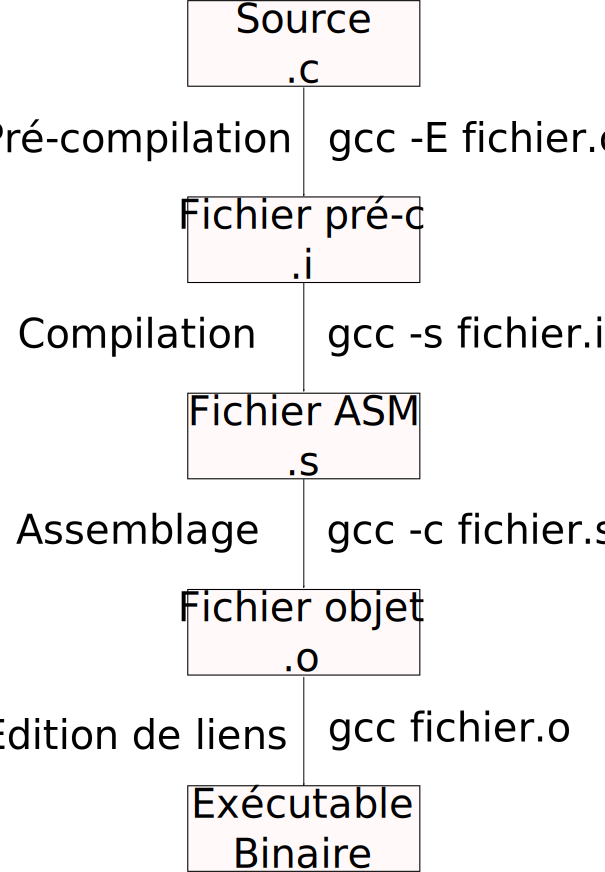
\includegraphics[height=.9\textheight]{images/source2bin.pdf}
\end{frame}

%!!!!!!!!!!!!!!!!!!!!!!!!!!!!!!!!!!!!!!!!!
\def\ftitle{Par la pratique}
\begin{frame}[containsverbatim]{\ftitle}
%_________________________________________
\def\blocktitle{En pratique}
\begin{block}{\blocktitle}
\begin{verbatim}
int main(void) {
  return 0;
}
\end{verbatim}
\end{block}

%_________________________________________
\def\blocktitle{gcc -c ops.c}
\begin{block}{\blocktitle}
\begin{itemize}
\item Créer le code ASM pour ce programme dans un fichier ops.o
\end{itemize}
\end{block}
%_________________________________________
\def\blocktitle{gcc }
\begin{block}{\blocktitle}
\begin{itemize}
\item gcc ops.o donne l'exécutable
\end{itemize}
\end{block}
\end{frame}


%!!!!!!!!!!!!!!!!!!!!!!!!!!!!!!!!!!!!!!!!!
\begin{frame}[containsverbatim]{\ftitle}
%_________________________________________
\def\blocktitle{Fichier supplémentaire}
\begin{block}{\blocktitle}
\begin{itemize}
\item On créer le fichier lmath.c contenant
\begin{verbatim}
int add(int a, int b) {
  return a + b;
}

int mul(int a, int b) {
  return a * b;
}
\end{verbatim}
\end{itemize}
\end{block}
%_________________________________________
\def\blocktitle{obs.c}
\begin{block}{\blocktitle}
\begin{verbatim}
#include "lmath.c"
int main(void) {
  int res = add(1, 2);
  res = add(2, 4);
  return 0;
}
\end{verbatim}
\end{block}
\end{frame}


%!!!!!!!!!!!!!!!!!!!!!!!!!!!!!!!!!!!!!!!!!
\begin{frame}[containsverbatim]{\ftitle}
%_________________________________________
\def\blocktitle{gcc obs.c}
\begin{block}{\blocktitle}
\begin{itemize}
\item Reviens à mettre toutes les fonctions dans le même fichier
\item Génère l'exécutable.
\end{itemize}
\end{block}


%_________________________________________
\def\blocktitle{Comment faire mieux?}
\begin{alertblock}{\blocktitle}
\begin{itemize}
\item On aimerai pouvoir compiler une partie de projet avec les fonctions add et mul et l'autre partie avec le main indépendamment.
\item Principe de la compilation séparée
\end{itemize}
\end{alertblock}
\end{frame}

%!!!!!!!!!!!!!!!!!!!!!!!!!!!!!!!!!!!!!!!!!
\begin{frame}[containsverbatim]{\ftitle}
%_________________________________________
\def\blocktitle{Compilation séparée}
\begin{block}{\blocktitle}
\begin{itemize}
\item gcc -c lmath.c
\item Génère un fichier lmath.o contenant le code des fonctions add et mul
\item Comme on ne veut pas inclure le code des fonctions dans obs.c, il faut créer un fichier d'en-têtes lmath.h
\begin{verbatim}
int add(int a, int b);
int mul(int a, int b);
\end{verbatim}
\item Ce fichier dit qu'il existe quelque part des fonctions nommées add et mul.
\end{itemize}
\end{block}
%_________________________________________
\def\blocktitle{obs.c}
\begin{block}{\blocktitle}\begin{verbatim}
#include "lmath.h"
int main(void) {
  int res = add(1, 2);
  res = mul(2, 4);
  return 0;
}
\end{verbatim}
\end{block}
\end{frame}


%!!!!!!!!!!!!!!!!!!!!!!!!!!!!!!!!!!!!!!!!!
\begin{frame}[containsverbatim]{\ftitle}

%_________________________________________
\def\blocktitle{gcc obs.c}
\begin{block}{\blocktitle}
\begin{itemize}
\item Erreur!!
\item Undefined reference to add...
\item Undefined reference to mul...
\item On a oublier de dire où se trouve le code assemblé de ces fonctions
\end{itemize}
\end{block}
%_________________________________________
\def\blocktitle{gcc lmath.o obs.c}
\begin{block}{\blocktitle}
\begin{itemize}
\item Compile obs.c en obs.o
\item Lie obs.o avec lmath.o et créer un exécutable.
\end{itemize}
\end{block}
\end{frame}


%!!!!!!!!!!!!!!!!!!!!!!!!!!!!!!!!!!!!!!!!!
\begin{frame}[containsverbatim]{\ftitle}
%_________________________________________
\def\blocktitle{Alternative}
\begin{block}{\blocktitle}
\begin{itemize}
\item gcc -c lmath.c
\item gcc -c obs.c
\item gcc obs.o lmath.o
\end{itemize}
\end{block}
\end{frame}


%!!!!!!!!!!!!!!!!!!!!!!!!!!!!!!!!!!!!!!!!!
\def\ftitle{Externe}
\begin{frame}[containsverbatim]{\ftitle}
%_________________________________________
\def\blocktitle{Variable externe}
\begin{block}{\blocktitle}
\begin{itemize}
\item Supposons que je souhaite avoir à ma disposition le dernier résultat calculé
\end{itemize}
\end{block}
%_________________________________________
\def\blocktitle{lmath.h}
\begin{block}{\blocktitle}
\begin{itemize}
\item Je définis la variable : \verb!extern int lastResult;!
\item Tout module qui importera lmath.h saura qu'il existe quelque part une variable nommée lastResult
\end{itemize}
\end{block}

%_________________________________________
\def\blocktitle{obs.c}
\begin{block}{\blocktitle}
\begin{verbatim}
#include "lmath.h"
int main(void) {
  add(1, 2);
  mul(lastRes, 4);
  return 0;
}
\end{verbatim}
\end{block}
\end{frame}


%!!!!!!!!!!!!!!!!!!!!!!!!!!!!!!!!!!!!!!!!!
\begin{frame}[containsverbatim]{\ftitle}
%_________________________________________
\def\blocktitle{Détails supplémentaires}
\begin{block}{\blocktitle}
\begin{itemize}
\item Lorsque l'on défini un prototype de fonction, il est extern implicitement!
\item Lorsque l'on défini une variable, elle ne l'est pas
\end{itemize}
\end{block}
\end{frame}



%!!!!!!!!!!!!!!!!!!!!!!!!!!!!!!!!!!!!!!!!!
\def\ftitle{Librairie}
\begin{frame}[containsverbatim]{\ftitle}
%_________________________________________
\def\blocktitle{Quand le répertoire prend l'o!}
\begin{block}{\blocktitle}
\begin{itemize}
\item Avec des grands projets, on se retrouve vite avec beaucoup de fichier .o
\item Pourquoi on ne pourrait pas les regrouper dans un seul package pour les lier en une fois
\item Et bien on peut grâce à ar
\item Tous les fichiers archivés dans une librairie : libXXX.a (ar -ra libXXX.a fichier.o / ranlib libXXX.a)
\item gcc fichier.c libXXX.a / gcc fichier.c -L. -lXXX
\item Exemple la bibliothèque standard c libc.a
\end{itemize}
\end{block}
\end{frame}

%!!!!!!!!!!!!!!!!!!!!!!!!!!!!!!!!!!!!!!!!!
\def\ftitle{Static sur la ligne!}
\begin{frame}[containsverbatim]{\ftitle}
%_________________________________________
\def\blocktitle{HelloWorld.c}
\begin{block}{\blocktitle}
\begin{verbatim}
#include <stdio.h>
int maint(void) {
  printf("Hello World\n");
  return 0;
}
\end{verbatim}
\end{block}
%_________________________________________
\def\blocktitle{Utilisation statique}
\begin{block}{\blocktitle}
\begin{itemize}
\item Le fichier header de stdio se trouve dans \verb!/usr/include!
\item Il indique que la fonction printf se trouve quelque part
\item gcc -static HelloWorld.c
\item Créer un programme standalone, qui contiendra le code de main, et celui de toutes fonctions appelées par printf.
\end{itemize}
\end{block}
\end{frame}


%!!!!!!!!!!!!!!!!!!!!!!!!!!!!!!!!!!!!!!!!!
\begin{frame}[containsverbatim]{\ftitle}
%_________________________________________
\def\blocktitle{C'est de la dynamique!}
\begin{block}{\blocktitle}
\begin{itemize}
\item On peut utiliser des librairies partagées par plusieurs programmes
\item Lors de l'exécution du programme, on fera la lisaison avec ses fonctions (dynamique)
\end{itemize}
\end{block}
%_________________________________________
\def\blocktitle{Exemple}
\begin{block}{\blocktitle}
\begin{itemize}
\item gcc -c -fPIC lmath.c
\item gcc -shared -o liblmath.so lmath.o
\item gcc -c main.c
\item gcc main.o -L. -llmath
\end{itemize}
\end{block}
\end{frame}

\end{document}
